% Auteur : Romain TESTUD
\begin{frame}{Les plate-formes d'échanges centralisés}
    \begin{block}{La solution la plus répandue}
        \begin{itemize}
            \item Achat / Vente / Échange de crypto-actifs.
            \item Intermédiaire entre les utilisateurs.
        \end{itemize}
    \end{block}
    \begin{block}{Interopérabilité ?}
        \begin{itemize}
            \item Utilisation de bridges inter-blockchains.
            \item Possibilité d'échanges entre tokens.
        \end{itemize}
    \end{block}
\end{frame}

\begin{frame}{Fonctionnement}    
    \begin{block}{Méthode de l'Order Book}
        \begin{itemize}
            \item Ordres d'achats.
            \item Offres de ventes.
        \end{itemize}
    \end{block}
        \centering
        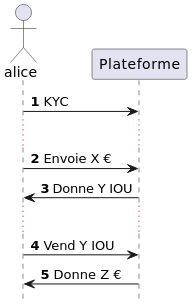
\includegraphics[scale = 0.5]{centralisation/img_plateformes/transaction.png}
\end{frame}

\begin{frame}{Avantages et inconvénients}
    \begin{block}{Avantages}
        \begin{itemize}
            \item Diverses fonctionnalités.
            \item Utilisation simplifiée.
        \end{itemize}
    \end{block}
    \begin{block}{Inconvénients}
        \begin{itemize}
            \item Sécurité et fiabilité relative au tiers.
            \item Gestion des données utilisateurs par le tiers.
            \item Fonctionnement interne opaque.
        \end{itemize}
        $\Rightarrow$ Confiance utilisateur/plate-forme.
    \end{block}
\end{frame}